
\chapter{WebTraceCollector}\label{ch:traceCollector}

To testing Websites and Mobile Applications, 
we use some devices to automatically generate traces.
The SpecElicitor is used for generating traces of Mobile Applications
and The WebTraceCollector is used for generating traces of Websites.
%為了測試APP和WEB,our lab使用了一些工具來產生traces

We make a tool named WebTraceCollector for automatically generating traces of Websites.
WebTraceCollector is write on Python and using Selenium as Library.
WebTraceCollector can explore the Website automatically with different algorithm,
generate traces with a finite state machine, which use the DOM\cite{DOM} tree of the web pages to construct.
WebTraceCollector can also work fine on the websites with Ajax Application,
and input texts on every input text fields with the fitting data.

%this paper 用python 和 seleium為基底建立一個可以自動explore website的trace collector
%此工具用DOM tree來做state-base的finite state machine

\section{Framework}

WebTraceCollector gets the URL of the Website as an input.
By setting configuration, User can make detailed rules like the max depths to explore on the Websites, the type of browser or the abstraction style of the DOM tree to explore the Websites precisely.

To manage all works, WebTraceCollector use a event list which records all events should be done.
WebTraceCollector pops out an event and implement the action of the event on the browser until there is no event on the event list.
After the action, it will check the current state of the browser by loading page source.
With the algorithm chosen by user, WebTraceCollector has different reaction with different situations.
The situations are entering a new state, entering an old state, keeping the same state and going out of the domain.
The algorithm of WebTraceCollector is shwon in Fig[].

\begin{algorithm}[htb]
	\begin{doublespace}		
		\KwIn{ URL, Config }
		Algorithm $\gets$ Config.getAlgorithm()\;
		Executor $\gets$ Config.getBrowser()\;
		InitialState $\gets$ Executor.initial(URL)\;
		\While{ EventList $\neq$ Empty }
		{
			Action $\gets$ EventList.getEvent()\;
			Executor.do(Action)\;
			NextState $\gets$ Executor.getState()\;
			\Switch{ NextState }
			{
				\Case{ SameState }
				{ Algorithm.staySameState() }
				\Case{ NewState }
				{ Algorithm.GotoNewState() }
				\Case{ OldState }
				{ Algorithm.GotoOldtate() }
				\Case{ OutOfDomain }
				{ Algorithm.OutOfDomain() }
			}			
		}		
	\end{doublespace}
	\caption{Overview}
	\label{algorithm:overview}
\end{algorithm} 

%此工具一邊使用selenium來操縱web browser,
%一邊建立state(DOM), edge(click ,inputs) 的automata
%此工具使用event list的形式,選擇一個algorithm,每次pop out一個待辦的event
%每次update:若是新的state,就將所有的clickables排入events,若是舊的state就無視

\clearpage

\section{Automata}

We construct an automata to represent the Website.
The state is defined based on the DOM tree of the web page.
If the URL, DOM tree or any element on the web page changes, we will recognize that it goes to other state.
The edge records one state goes to another state by an action,
which clicks the specific clickable tag with values written in all form elements.
The web page of automata is shown in Fig[\ref{AutomataOverview}].

As the test result, WebTraceCollector generates traces information in different types of files. 
There are JSON files of traces and automata, screenshots of every state, DOM tree and detail information of every state and a web page of overview automata.
Automata.json records all states, which have URL, ID, screenshot and DOM tree of the web page, and edges.
Traces.json records the states and edges with the order
The example of the test result is shown in Fig[\ref{TestResult}].

\clearpage

\begin{figure}[h]
	\graphicspath{{pic/}}
	\begin{center}
		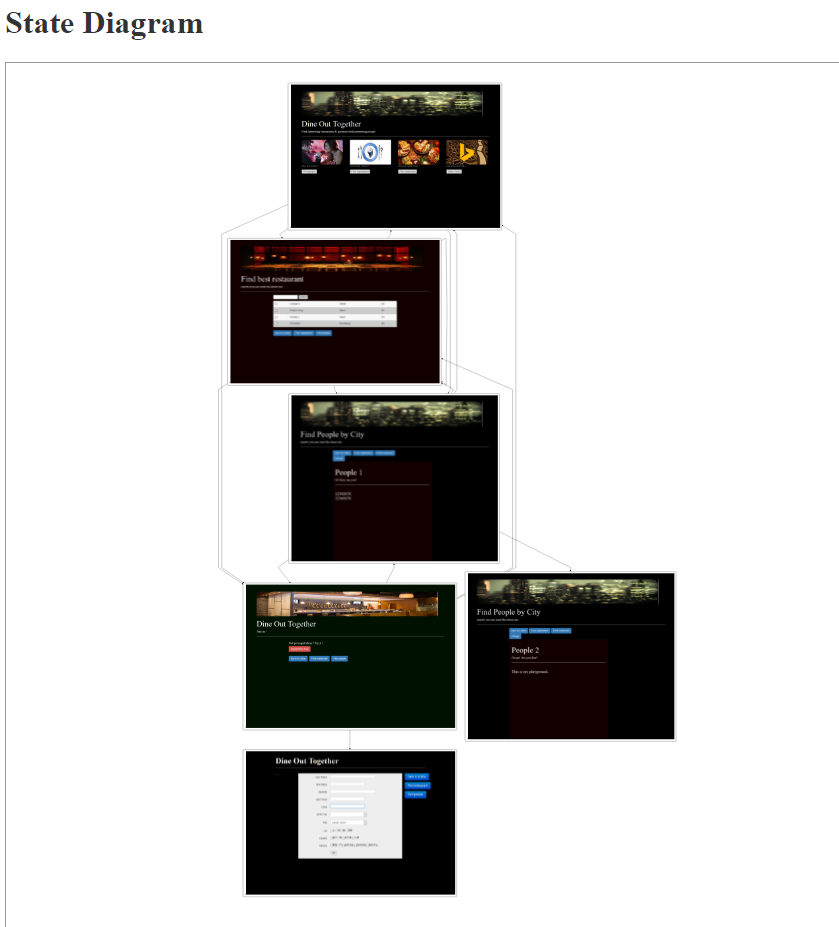
\includegraphics[width=0.6\textwidth]{automata_overview.png}
	\end{center}
	\caption{ Overview of the Automata. }
	\label{AutomataOverview}
\end{figure}

\begin{figure}[h]
	\graphicspath{{pic/}}
	\begin{center}
		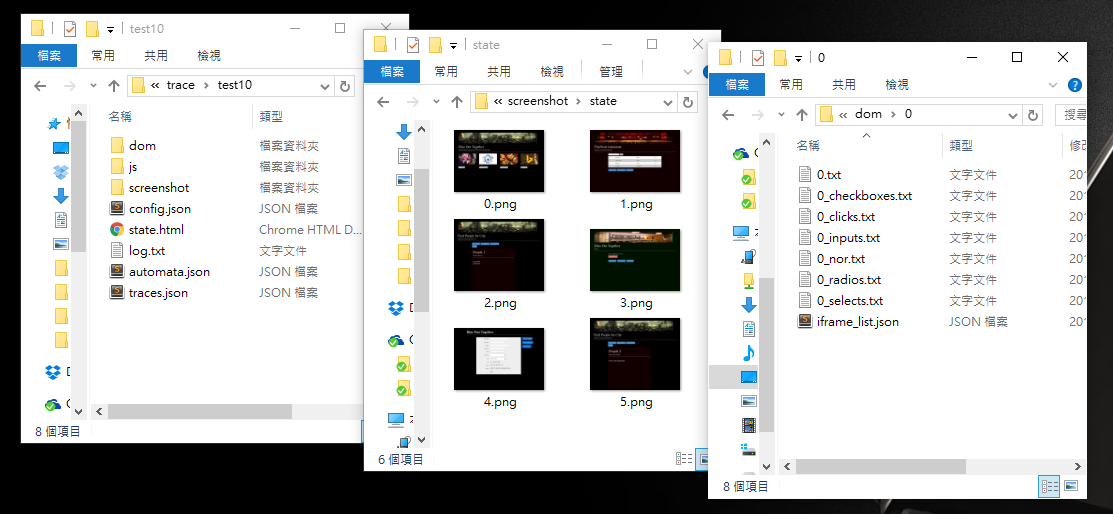
\includegraphics[width=0.8\textwidth]{webTraceResult.png}
	\end{center}
	\caption{An Example traces of the website. }
	\label{TestResult}
\end{figure}

%一個element:有clickable,input,radio,checkbox,select
%一個state:有ID,dom list,all elements,all clickable
%其中DOM又含有iframe的結構
%一個edge:有ID,from to state,all elements with value,one clickable
%一個trace:有states edges照order排

\clearpage

\section{Event}

During the testing, WebTraceCollector repeats getting an event from the event list and implement the action of the event until the event list is empty.
An event consists of action, state and depth.
The action implies which clickable element should be clicked.
The state implies where the element locates in.
The depth implies how deep this event is in the automata.
Before the action, WebTraceCollector checks the current state on th browser is equal to the state recorded on the event.
If not, the automata finds a simple path to the target state and make the browser go to the correct state.

To work fine on the websites that not only have buttons to click but also have form elements,
WebTraceCollector needs to insert values into those elements when it implements the clicking action.
The elements are inputs, selects, radios and checkboxes.
Because the Website may only accept certain words as input values likes , we cannot just make random string to test the Website,
we construct a database to analysis the element and find the most suitable string.
The database has some example values of the common inputs we generalize from websites.
Considering the element's tag, id, name and other siblings tags,
WebTraceCollector will use the most similar string to the examples as the input value of the element.
The algorithm of implementing the action is shwon in algorithm[\ref{algorithm:action}].

%要執行click action時,會先對所有的input 填值,會連上database進行input,clickable的tag等feature的字串處理,找出推薦的適當的值填入

\begin{algorithm}[htb]
	\begin{doublespace}		
		\KwIn{ action, state, depth }
		\If{ CurrentState $\neq$ state }
		{
			BackTrack( state )\;
		}
		Clickable $\gets$ action.getClickable()\;
		Inputs, Selects, Radios, Checkboxes $\gets$ state.getFormElements()\;
		\ForEach{ Element in Inputs, Selects, Radios, Checkboxes }
		{
			Value = Database.findValue( Element )\;
			Executor.setValue( Element, Value )\;
		}
		Executor.click( Clickable )\;
		
	\end{doublespace}
	\caption{To implement the action}
	\label{algorithm:action}
\end{algorithm} 

\clearpage

\section{normalization}

After the action, WebTraceCollector will check what happens on the browser by comparing the current state of the web page and other states in the automata.
The states have the information of DOM tree loading from the browser by Selenium.
However, ther are some problems if we just take two DOM trees as strings to compare.
For example, there may be advertising applications, calender, popularity or catalogs shown on the website.
Each time user visits the website, the DOM tree of the website may be different.
To prevent recognizing a wrong state, we must preprocess the DOM tree.

The work of preprocessing is removing the elements that may confuse us and remain the elements we want to focus on.
We remove the tags that are unvisible on the web page, the javascripts code, the HEAD of the html and the css style.
We construct a class named normalizer, which can scan the DOM tree, find the target element and remove it.
For specific website, User can set the specific normalizer to normalize the DOM tree by his own style.
The examples of DOM tree and normalized DOM tree are shown in Fig[\ref{DOMvsNorDOM}].

%state用DOM比較,但有問題需要省略
%省略的方式有config

\begin{figure}[h]
	\graphicspath{{pic/}}
	\begin{center}
		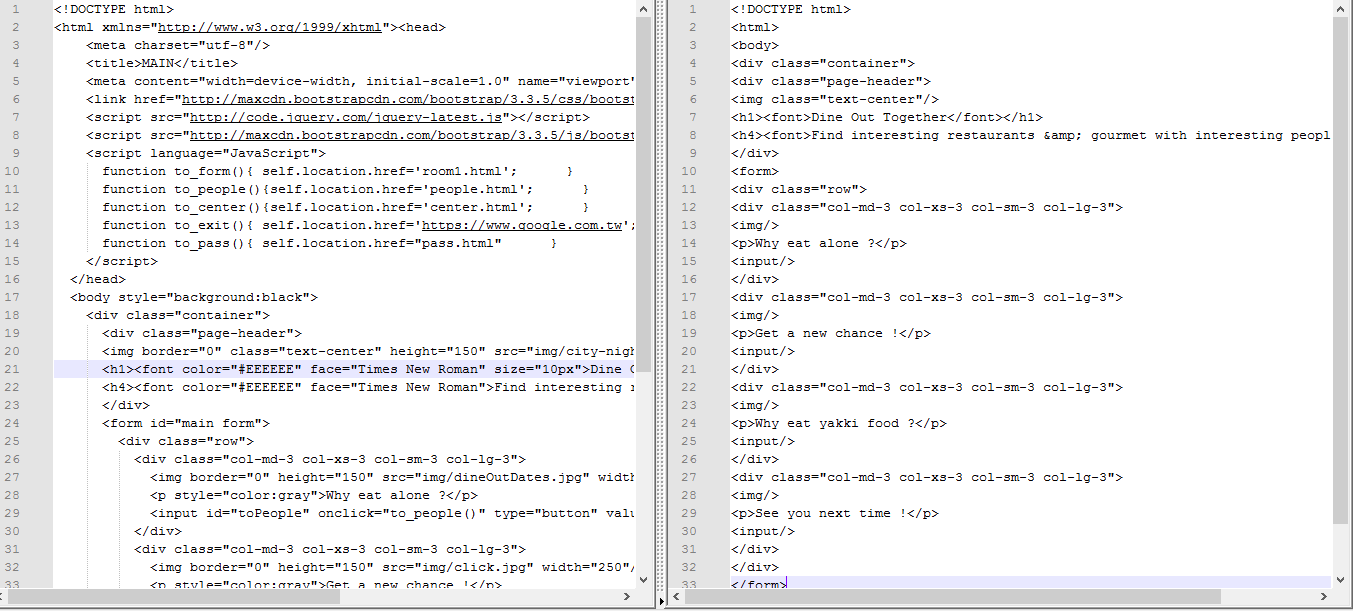
\includegraphics[width=0.8\textwidth]{DOMvsNorDOM.png}
	\end{center}
	\caption{An Example of DOM tree compare with Normalize DOM tree. }
	\label{DOMvsNorDOM}
\end{figure}

\clearpage

\section{Algorithm}

WebTraceCollector can explore the website with algorithm set by user.
We make Three algorithms for WebTraceCollector: Monkey, DFS and CrossBrowser.
User can choose the algorithm and set to the config as an input before starting the test.
WebTraceCollector will switch it's reaction by the algorithm at every stage after action during the test.

%根據不同的algorithm,此工具面對可按的clickables

\subsection{Monkey}

The monkey algorithm simply adds a random event to the event list.
Every time when WebTraceCollector detects the DOM tree changed and encounters a different state,
it collects all clickable elements from the current state and randomly choose one as next event.
User can set the trace length and trace amount in the config,
which means the maximum edges in one trace and the total amount of all traces.
The example overview of a monkey traces is shown in Fig[\ref{MonkeyAutomata}].
The trace generated by monkey algorithm may contains a loop, 
because monkey algorithm may choose the same clickable.

\begin{figure}[h]
	\graphicspath{{pic/}}
	\begin{center}
		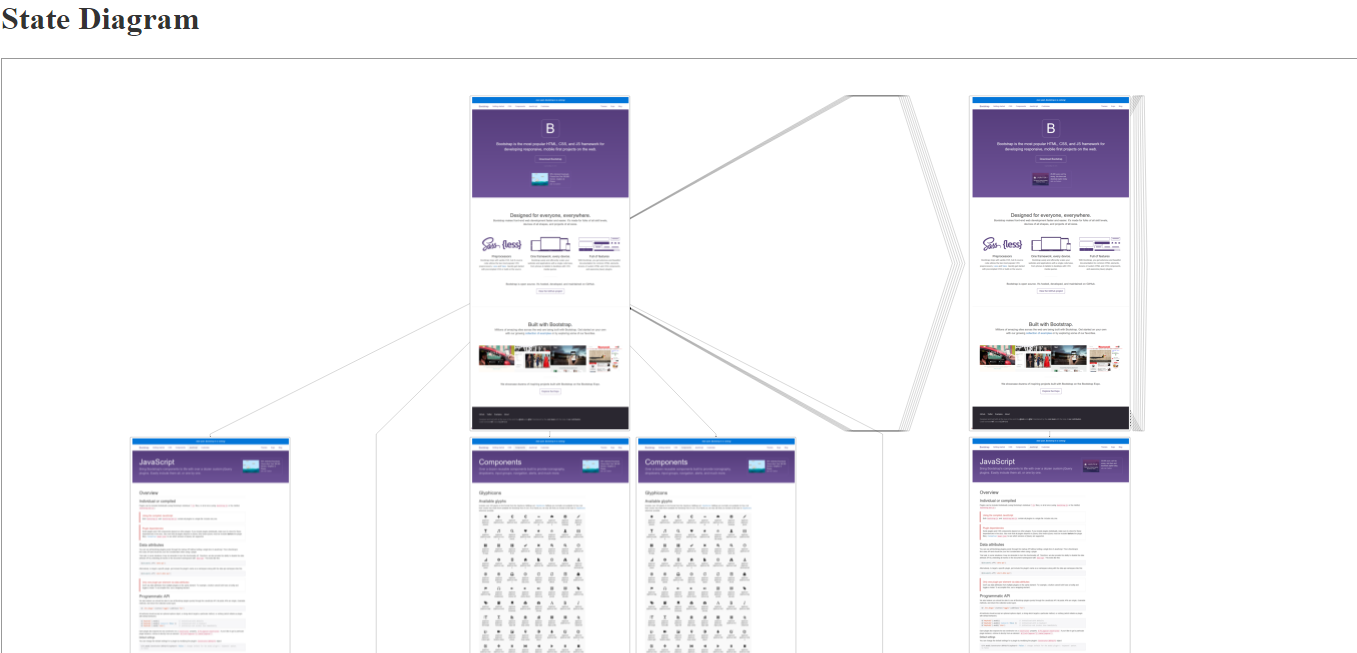
\includegraphics[width=0.8\textwidth]{MonkeyAutomata.png}
	\end{center}
	\caption{An Example of Monkey traces. }
	\label{MonkeyAutomata}
\end{figure}

%每次update:在length max以前,在現在state可見的clickables中隨機挑一個排入events

\subsection{Depth First Search}

The disadvantage of monkey algorithm is that it may only visit certain web pages and not explore the whole website.
To guarantee all clickable elements will be clicked durring the testing,
We develop the DFS algorithm.
However, Some Websites is too huge to explore all of it's web pages, like Wiki or News,
or too complicated that makes unlimited different web pages, like chat room or other dynamic websites. 
User has to set the maximum depth of the DFS,
so the DFS algorithm only explore the website with the depth from the initial web page less than the max depth.
The example overview of a DFS traces is shown in Fig[\ref{DFSautomata}].

Unlike the Monkey algorithm, DFS algorithm adds all evenst on the current state to the event list.
When WebTraceCollector encounter a different web page,
it will download the page source of the web page as a state and compare the current state with other states in the automata.
For the four different situations mentioned before,
the DFS algorithm has different reaction.
If the current state is a new state, which means this web page does not visited before,
this state will added into the automata and all clickable elements will made as an event and added into the event list.
If the currenrt state is an old state or is as same as the last state,
there will be no new events added and continue next event.
If the URL is out of the domain, WebTraceCollector will ignore this state and back to the last state.

\begin{figure}[h]
	\graphicspath{{pic/}}
	\begin{center}
		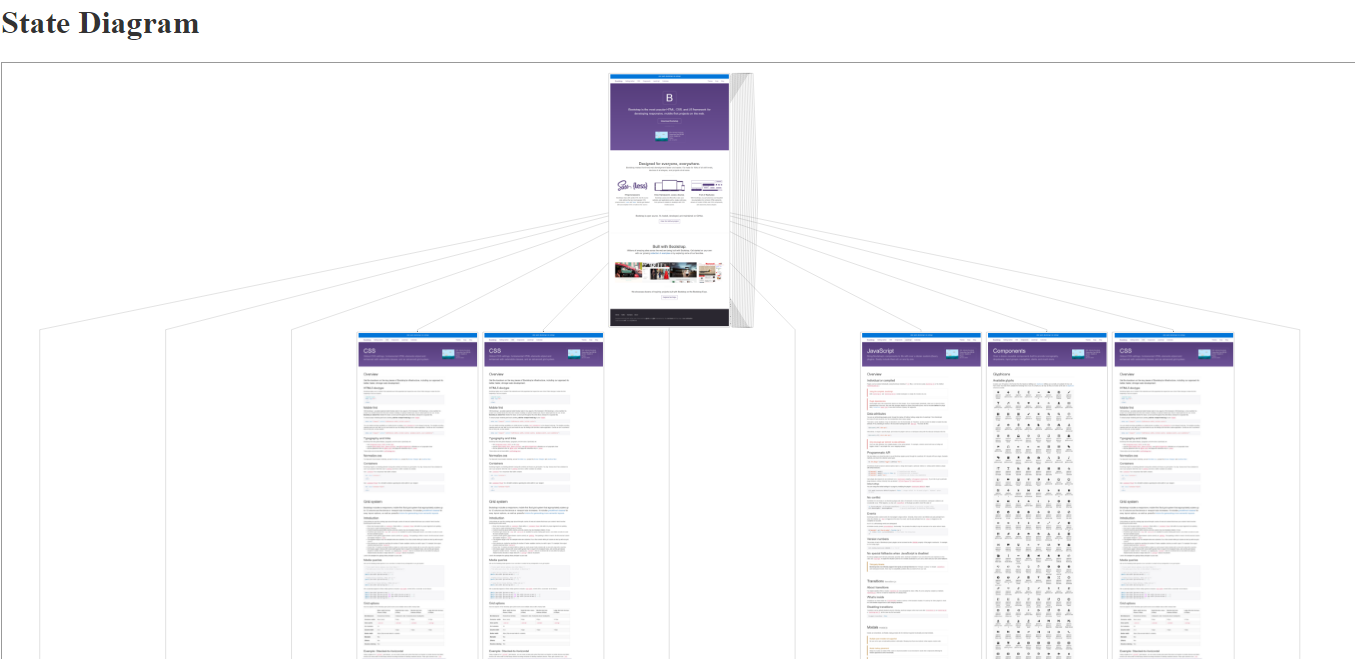
\includegraphics[width=0.8\textwidth]{DFSautomata.png}
	\end{center}
	\caption{An Example of DFS traces. }
	\label{DFSautomata}
\end{figure}

\clearpage

